\documentclass[10pt]{beamer}

\usepackage{appendixnumberbeamer}

\usepackage{booktabs}
\usepackage[scale=2]{ccicons}

\usepackage{pgfplots}
\usepgfplotslibrary{dateplot}

\usepackage{xspace}
\usepackage{../theme_style}
\setbeameroption{show notes}

\title[Context Awareness]{Exam question six - Context Awareness}
\subtitle{Distributed and Pervasive Systems}
\date{June 03, 2022}
\author[M.H. Kristensen]{Morten Haahr Kristensen}
\def\studentid{201807664}
\institute{Department of Electrical and Computer Engineering - Aarhus University}
% Logo only on title page
\titlegraphic{
    
\includegraphics[width=12cm]{figs/aulogo_big.png}
}
\begin{document}

\maketitle

\begin{frame}{Outline}
  \setbeamertemplate{section in toc}[sections numbered]
  \tableofcontents[hideallsubsections]
\end{frame}

\section{Concepts}

\begin{frame}
  \frametitle{Pervasive Systems}
  Pervasive systems definition: \\
  \vspace*{-1.0em}
  \begin{quote}
    \textbf{Pervasive systems} are context-aware sensor-based \textbf{systems} which are \textbf{inspired} by \textbf{pervasive computing concepts}, methods and best practices, and which \textbf{relies} on \textbf{pervasive enabling technologies} to \textbf{achieve} a \textbf{calm}, \textbf{effective}, and \textbf{efficient} technology experience for their users. (Wagner 2022 \cite{wagnerPervasiveComputing2022})
  \end{quote}
  \note{
    Difference between pervasive computing and pervasive systems:\\
    Pervasive system is the architecture.\\
    Pervasive computing is the technique (how it is done).

    Calm technology: A technology that is designed to mainly occur in the user's periphery. The information only presents itself when needed and otherwise stays calmly on the user's periphery. 
    }
\end{frame}

\begin{frame}
  \frametitle{Smart stuff}
  Smart device
  \vspace*{2em}

  Smart environment
  \vspace*{2em}

  Smart space
  \vspace*{2em}

  Smart interaction
  
  \note{
    \footnotesize
    When talking about pervasive systems it is inevitable to run across the ''smart stuff''. We generally talk about three categories of smart x:\\
    Smart device: An electronic device that can connect, share and interact with a pervasive system. I.e. other smart devices. \\
    Smart environment: An environment that can acquire and apply knowledge, through smart devices, about the environment and its users to improve their experience.\\
    Smart space: A smart space is a smaller area of a smart environment.\\
    A smart environment could be a hospital where the ventilation is automated, bed occupancy is tracked, and the nearest doctor is automatically called for if an emergency happens if he is not busy. A smart space in the hospital could be a specific room where the screen automatically opens the patients' journal when the nurse enters.\\
    Smart interaction: Dynamic organization and interaction between components to achieve shared goals. Can be internal or driven by external events.
  }
\end{frame}

\begin{frame}
  \frametitle{Context}

  \begin{quote}
    Any \textbf{information} that can be used to \textbf{characterize} the situation of an \textbf{entity}. An entity is a person, place, or object that is considered \textbf{relevant} to the interaction between a user and an application, including the user and the applications them-selves. (Dey 2010)
  \end{quote}

\end{frame}

\section{Context Awareness}

\begin{frame}
  \frametitle{Definition}
  \begin{quote}
    A system is context-aware if it uses context to provide relevant information and/or services to the user, where relevancy depends on the user's task. (Dey 2010)
  \end{quote}
\end{frame}

\begin{frame}
  \frametitle{Context life cycle model}
  \begin{figure}
    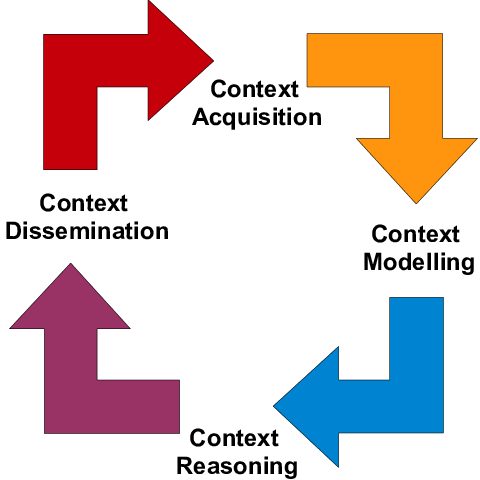
\includegraphics[width=0.5\textwidth]{figs/context_life_cycle_model.png}
    \caption{Context life cycle model. ''The simplest form of a context life cycle''. Quote and figure: \cite{pereraContextAwareComputing2013}}
  \end{figure}
  \note{
    The context life cycle model shows the minimum steps required in making a context-aware system. \\
    Acquisition: We acquire some sort of data from a sensor. Could be a light sensor. \\
    Modeling: We put it into the model that we built. Could be a linear regression in this case. \\ 
    Reasoning: We make a decision. The light should be off as the room is bright already. \\
    Dissemination: We act on the decision. Turn off the light if it is on or do nothing if it is off.
  }
\end{frame}

\begin{frame}
  \frametitle{Context Awareness challenges}

  Selected challenges with context-awareness\footnote{Inspired by: \cite{wagnerContextAwareness2022}.}:
  \begin{itemize}
    \item Classification errors in context models
    \item Edge cases are hard to deal with
    \item Sensor fidelity
    \item Complex contexts with interrelated moving parts
    \item Generation of huge amounts of data
    \item User privacy
  \end{itemize}
  \note{
    \footnotesize
    Classification and edge cases: It can be really hard to make a good context model. Especially if you have to take the edge cases into account. For instance what if the system is tracking presence through a PIR sensor but the user is sitting very still. What if this activated the alarm so the next time he moves it turns on? \\
    Sensor fidelity: Our data sources only have a certain fidelity and we have to try and make a complete context model despite their limitations. If you are tracking with PIR sensors, how do you know it is the same person you are tracking? \\
    Data: I remember Qi, our WSN lecturer, talking about how much data generation would be required for fully autonomous cars in the city. I don't remember the exact amount but it was very high. And they would have to share that from car to car. \\ 
    Privacy: In session 6 we learned about how easily a person's position could be extrapolated from cellphone data although it was anonymized. Imagine what one can do if the entire house is collecting data.
  }
\end{frame}

\begin{frame}
  \frametitle{Accuracy vs. Costs}
  \begin{figure}
    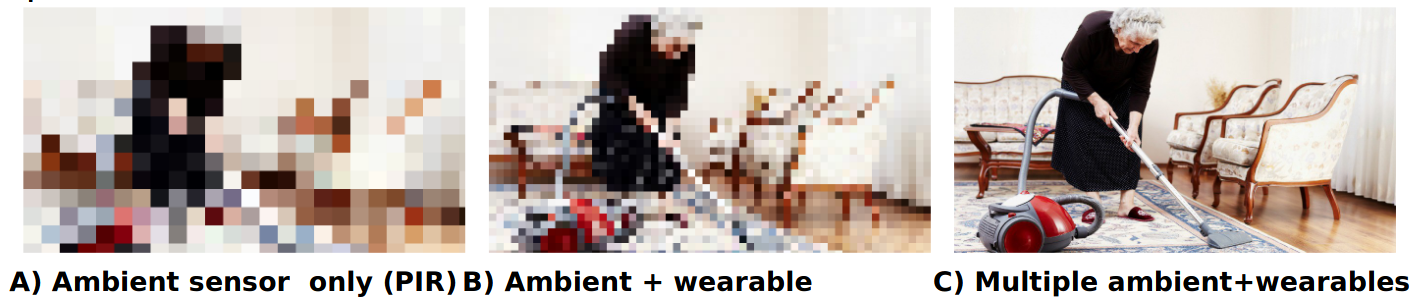
\includegraphics[width=\textwidth]{figs/accuracy_vs_costs.png}
    \caption{Example of a low cost vs. high cost system. Image: \cite{wagnerContextAwareness2022}}
  \end{figure}
  \note{
    Often determining the context boils down to a classification problem of some sort. This is where pervasive systems require a lot of experimentation. How big a cost is needed for the sensors that we use in our system? Can we get away with using a simple PIR sensor like in the first picture? Or do we need multiple ambient sensors? \\ 
    The end problem always boils down to a cost-benefit problem. We can always make our product more accurate by investing more.
  }

\end{frame}

\section{Development}

\begin{frame}
  \frametitle{Network technologies}
  \begin{figure}
    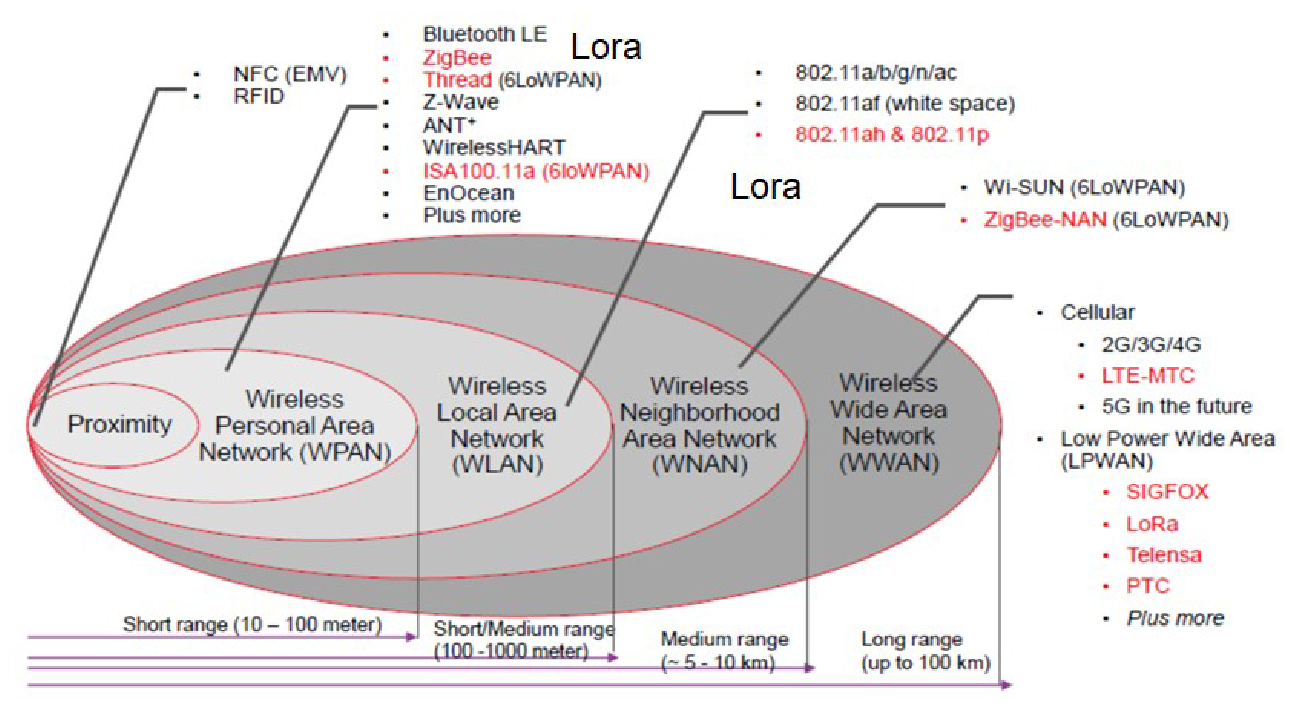
\includegraphics[width=0.8\textwidth]{figs/network_technologies.png}
    \caption{Different network technologies. Image: \cite{wagnerContextAwareness2022}}
  \end{figure}
  \note{
    One of the first things you should look at is which network technology you want to use. The biggest difference between these is the ranges and from there it might depend on which smart devices you wish to incorporate. E.g. if you already have sensors that use ZigBee it might make sense to keep using that.\\
    During our project, we had a mixture of technologies, which is also possible, but in this case, it was mainly for educational purposes. We used WiFi for our control units, Bluetooth for a speaker and ZigBee for various sensors. The control units mainly used MQTT for the application layer where a ZigBee2MQTT converter allowed us to communicate with the sensors. We also used HTTPS requests with JSON content to communicate to the Alexa cloud services.
  }
\end{frame}

\begin{frame}
  \frametitle{Prototyping}

    \begin{figure}
    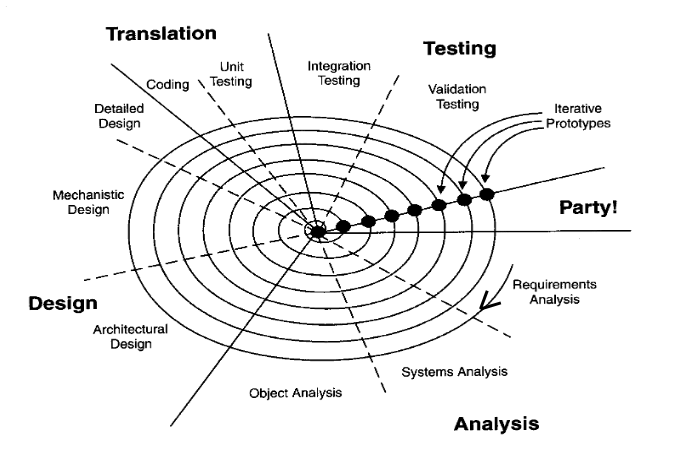
\includegraphics[width=0.9\textwidth]{figs/iterative_prototyping.png}
    \caption{Model for iterative prototyping. Image: \cite{wagnerPervasiveComputing2022}.}
  \end{figure}
  \note{
    Perhaps the most important method for building a pervasive system is to do prototyping with extra focus on the testing phase. We already talked about accuracy vs. cost and to ensure that you pick the optimal choice, it is necessary to test many different solutions. \\
    Especially the validation test can be important. When we did our project we only did one iteration, and we thought our end solution was great. We then did some validation testing on what we considered the end-users, i.e. other engineering students, and most of them didn't like it. One of the main reasons was that the system included a camera, which meant constant surveillance of their home.
  }
\end{frame}

\section{Towards intelligent environments}
\begin{frame}[standout]
  \frametitle{Towards Intelligent Environments}
  % \centering
  Keep moving forward...

  \footnotesize
  ... and maybe standardize more things.
  \note{
    % \footnotesize
    We are getting there. Especially in the medical sector, there is a lot of research going on. But I think one of the big challenges is that the companies are not opening up their services enough to allow for intelligent environments to be truly smart. And why would they? It's probably a lot more profitable to lock the buyers into your ecosystem so that the hospital has to keep reinvesting in your equipment instead of the competitors. So I think to truly get intelligent environments the users need to start making requirements for the vendors to make their devices compatible with each other. This could be done by standardizing what different devices provide, similar to what the Zigbee2MQTT library does.\\
    We are seeing increasing compatibility with the apps like ''Home Assistant'', ''Google Home'', etc. where you can register your device in there to control them. But then we are mainly still limited to controlling them through apps and not smart interactions.
  }

\end{frame}


\section{References}
\begin{frame}[allowframebreaks]{References}
  \bibliographystyle{ieeetr}
  \bibliography{references}
\end{frame}
\end{document}
